\documentclass[12pt]{report}
\usepackage[utf8]{inputenc}
\usepackage{amsmath}
\usepackage{amsfonts}
\usepackage{amssymb}
\usepackage{graphicx}
\usepackage{caption}
\usepackage{booktabs}
\usepackage{hyperref}
\usepackage{subfig}
\usepackage[acronym]{glossaries}

\newglossaryentry{cnn}{name=cnn,description={Convolutional Neural Network}}
\newglossaryentry{adt}{name=adt,description={Atlantic Daylight Time}}
\newglossaryentry{est}{name=est,description={Eastern Standard Time}}

%
\title{Reinforcement Learning Based Navigation with Semantic Knowledge of Indoor Environment}	%% title
\author{NGUYEN, Tai Long}			%% author's name

%
\newcommand{\argmax}{\arg\!\max}

\makeglossaries

\begin{document}
%
\maketitle
\tableofcontents

%
\chapter*{Acknowledgements}

First of all, I would like to express my sincere thanks to my advisor Dr. Nguyen Do Van for his support and guidance throughout this research work. I would also like to thank teachers and members of Human Machine Interaction Laboratory of University of Engineering and Technology for their help. Because time is limited and this research inevitably has shortcomings, I look forward to the comments of the teachers for future improvements.

%
\listoffigures
\listoftables
%

\chapter{Introduction}
In this chapter, I will briefly introduce the problem, the related works and state out the major contributions of this research.


\section{Problem Definition}

Robot navigation is referred to the problem where a robot is taught, or trained, to navigate smoothly in an environment in order to reach a particular targeted position. In other words, the learning robot must not collide to any obstacle or get stucked in a loop when moving around. Due to the multi-spectral applications, robot navigation has long been one of the most important tasks when it comes to deploying machine learning systems in real world.

\section{Related Works}
Enabling robots to autonomously navigate in complex environments is essential. Prior methods approached this problem by having the robot to maintain an internal map of the world, and then use a localization and planning method to navigate through that map. However, not only these approaches often include a variety of assumptions, but they are also computationally intensive due to high sample complexity. Meanwhile, deep neural networks demonstrated some success in navigational tasks, directly predicting actions from raw pixel observations of an agent. An obvious drawback of this class of models is their demand for supervision, while collecting training data for navigational tasks is tedious and labour intensive. Fortunately, learning to navigate can also be formulated by Reinforcement Learning, the algorithm which allows an agent to learn in a self-supervised manner by trial-and-error, guided only by a reward function. 

In the past few years, several RL-based methods have been introduced to solve this problem effectively on both real-world and simulated environments. Yuke Zhu et al  \cite{yuzhu} proposed a method that uses both current observation and image of target as input of the neural network so it can learn to behave in different scenes and find novel objects. Despite promising performance, the input pipeline that requires collecting images of target might be inefficient when applying to real world.

Also aiming for training an agent that can navigate and find different objects in different scenes, Ii Yang et al \cite{iiyang} aggregated Graph Convolutional Network and semantic text embedding to further enhance its generalization. The encoding the relationships between objects given by the graph significantly increases the performance of model compared to vanilla famous A3C. However, the authors used classification scores pretrained on ImageNet \cite{imagenet} dataset, which is not fully-customized for any specify set of training, indicating that there are rooms left for improvement. 

\section{Main Contribution}

Extending the idea of \cite{iiyang}, this work also integrates Graph Convolutional Network into learning algorithm. However, the input feeded to graph is object detection information rather than classification scores.
\newpage\cleardoublepage
\chapter{Background}
In this chapter, I will go through some background knowledge needed to better understand this work.

\section{Deep Reinforcement Learning}
In recent years, Deep Reinforcement Learning has gradually become one of the most active research areas in machine learning and artificial intelligence. The core idea of Reinforcement Learning is learning by trial and error: the model becomes better while interacting with environment. Roughly speaking, Reinforcement Learning lies somewhere in between supervised and unsupervised learning. While supervised learning requires a target label for each training example and unsupervised learning needs no labels at all, Reinforcement Learning uses sparse and time-delayed labels, the rewards, based on which the agent learn to behave correctly in the environment. This learning procedure is somehow similar to the model of how human beings learn in the real world. 

To put it into formalization, Reinforcement Learning can be modeled as a \textbf{Markov Decision Process} (MDP) represented by the tuple $<S, A, P, R, \gamma>$, where:
\begin{itemize}
\item $S$ is a set of environment states with Markov property.
\item $A$ is a set of possible actions.
\item $P$ is transition matrix (transition dynamics) and $P^a_{ss'} = P[S_{t+1} = s' | S_t = s, A_t = a]$.
\item $R$ is a reward function.
\item $\gamma$ is the discounted factor whose value lies in the interval $[0, 1]$.

\end{itemize}

To navigate in the environment, training agent uses a policy to choose the next action, which is defined by the function $\pi$, a mapping from state to action and can be either deterministic or stochastic:
\begin{itemize}
\item Deteministic: $\pi(s) = a$.
\item Stochastic: $\pi(a|s) = P_{\pi}(A=a|S=s)$.
\end{itemize}

One episode of this process (e.g. one game) forms a finite sequence of states, actions and rewards, defined as $H = (s_0, a_0, r_1, s_1, a_1, r_2, .., s_T, a_T, r_{T+1})$. To evaluate the performance of a agent in the environment, we use the total discounted future reward after the timestep $t$ of one episode, also kwown as $return$, which is calculated by:
\begin{align}
G_t &= R_{t+1} + \gamma R_{t+2} + \dots = \sum_{k=0}^{\infty} \gamma^k R_{t+k+1}
\end{align}

The discounting factor $\gamma \in [0, 1]$ is used to penalize the rewards in the future. To measure the goodness of a state, we use a \textbf{state-value} function defined as:

\begin{align}
V_{\pi}(s) &= \mathbb{E}_{\pi}[G_t \vert S_t = s]
\end{align}

Similarly, we define the \textbf{action-value} function of a state-action pair as:

\begin{align}
Q_{\pi}(s, a) &= \mathbb{E}_{\pi}[G_t \vert S_t = s, A_t = a]
\end{align}

The difference between action-value and state-value is called \textbf{action advantage} function:

\begin{align}
A_{\pi}(s, a) &= Q_{\pi}(s, a) - V_{\pi}(s)
\end{align}

The Reinforcement Learning algorithms are primarily concerned with how to obtain the optimal policy $\pi^*$, which maximizes the function $V_{\pi}(s)$ for all starting states, in both cases when the environment model, i.e. transition dynamics, is known or unknown. The agent must interact with the environment directly to obtain information which then is used by an appropriate algorithm to gradually turn its policy to an optimal one.

\begin{figure}
\centering
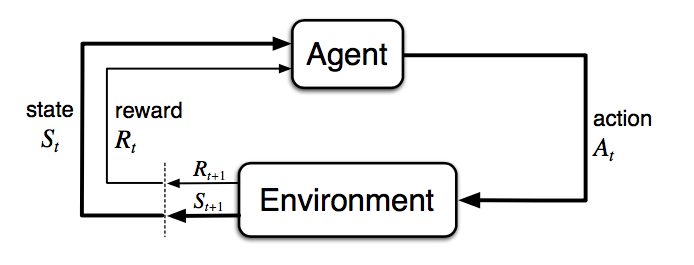
\includegraphics[scale=0.4]{charts/agent_environment_MDP.png}
\caption{The agent-environment interaction in a Markov decision process.}
\end{figure}

\section{Policy Gradient}

In order to solve a MDP, different approaches have been introduced and developed. Whereas iterative methods, such as value iteration or policy iteration, aim to learn the state-value function and then use it to produce the optimal policy, policy gradient methods directly learn the optimal policy with a parameterized function respect to $\theta$: $\pi_{\theta} = \pi(a|s;\theta)$

We define a reward function (opposite of loss function of traditional classification problems in machine learning) as the expected return and train the algorithm with the goal to maximize the reward function, which is defined as:

\begin{align}
\mathcal{J}(\theta) &= \sum_{s \in \mathcal{S}} d_{\pi_\theta}(s) V_{\pi_\theta}(s) = \sum_{s \in \mathcal{S}} \Big( d_{\pi_\theta}(s) \sum_{a \in \mathcal{A}} \pi(a \vert s, \theta) Q_\pi(s, a) \Big)
\end{align}

where $d_{\pi_{\theta}}(s)$ is stationary distribution of Markov chain for $\pi_{\theta}$. The gradient of the reward function respect to its parameters is calculated by:

\begin{align}
\nabla \mathcal{J}(\theta) &= \mathbb{E}_{\pi_\theta} [\nabla \ln \pi(a \vert s, \theta) Q_\pi(s, a)] \label{gradient}
\end{align}

In fact, Schulman et al., \cite{schulman} stated out several different expressions that policy gradient can be expressed and all of them share the same formula:

\begin{align}
\nabla \mathcal{J}(\theta) &= \mathbb{E} \left [ \sum^{\infty}_{t=0}\Psi_t \,\nabla \log \pi_{\theta}(a_t | s_t) \right ]
\end{align}

where $\Psi_t$ could be one of the following forms:

\begin{itemize}
\item $\sum^{\infty}_{t=0} r_t$: total reward of a episode.
\item $\sum^{\infty}_{t=t'} r_{t'}$: total reward of a episode following the action $a_{t'}$.
\item $\sum^{\infty}_{t=t'} r_{t'} - b_{t'}$: baselined version to reduce variance without introducing new bias to the estimation.
\item $Q_{\pi}(s_t, a_t)$: state-action value function.
\item $A_{\pi}(s_t, a_t)$: advantage function.
\item $r_t + V_{\pi}(s_{t+1}) - V_{\pi}(s_t)$: temporal difference residual.
\end{itemize}

By running the agent(s) and collect a large number of episodes, we can estimate the gradient and use gradient ascent algorithm to find the best $\theta$ we need.

\section{Actor Critic}

Vanilla policy gradient methods suffer from high variance thus leading to low convergence in many problems. Actor-critic algorithm tackles this problem by learning both value function and policy model at the same time. This strategy makes a lot of sense since knowing the value function leads to more accurate policy update. Actor-critic methods consist of two neural networks:

\begin{itemize}
\item Critic: updates the value function with gradient descent in a supervised manner, which could be state-value or action-value.
\item Actor: update the policy in the direction suggest by the critic using equation \ref{gradient}
\end{itemize}

These two neural networks are updated constantly in the training phase while together assisting agent to interact with environment. To further increase the effectivity and efficiency of Actor-Critic algorithm, Mnih et al. \cite{mnih} introduced Asynchronous Advantage Actor-Critic, or A3C, with a special focus on parallel training. In A3C, multiple agents run in their own copy of environments with a copy of the global network, gather samples, calculate and accumulate gradients needed and then perform the asychronous updates. From optimization perspective, the gradient accumulation step can be considered as a parallelized reformation of minibatch-based stochastic gradient update. 

\begin{figure}
\centering
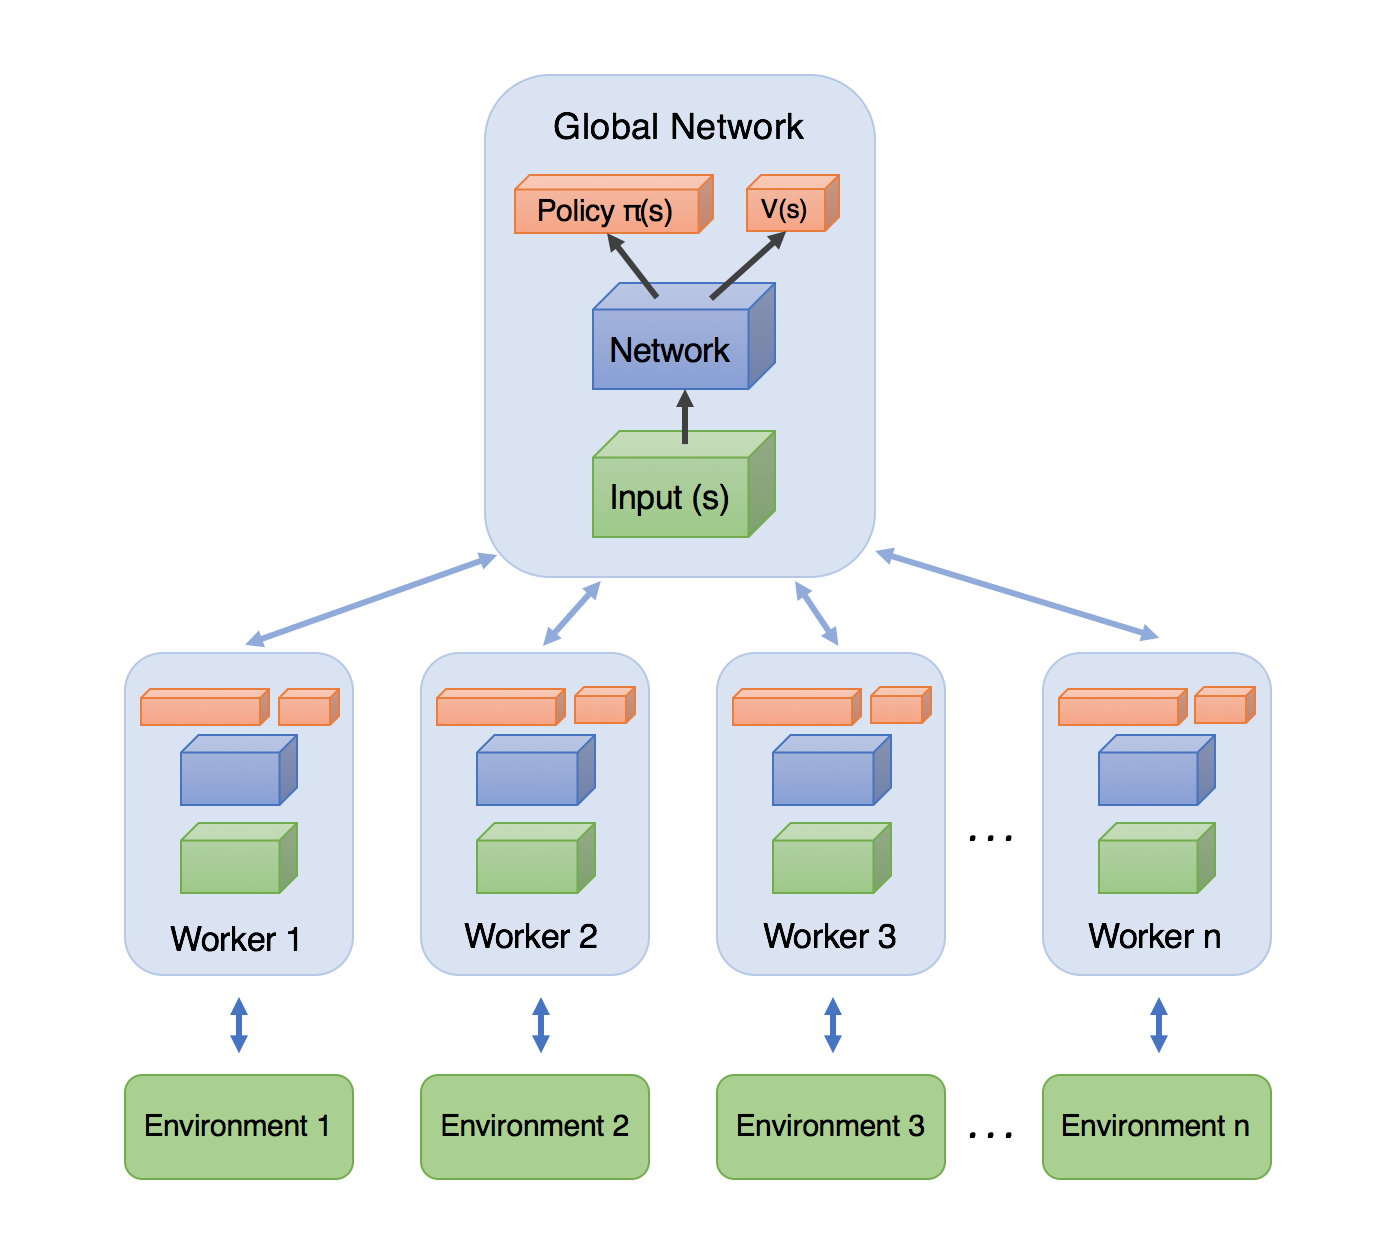
\includegraphics[scale=0.2]{charts/a3c.png}
\caption{The work flow of A3C algorithm.}
\end{figure}

The synchronous version of A3C is A2C, which has a coordinator that waits for all the agents to finish their work before updating the global parameters so that in the next training iteration they start with the same policy. A2C has been shown to utilize GPUs more efficiently and work better with large batch sizes while achieving same or better performance than A3C.

\section{ResNet-50 Network}
Of all machine learning techniques leading to the success of Deep Learning, or more specifically in Computer Vision,\gls{cnn} is known as the most essential one. Recent years have been witnessing a constant raise in top accuracies in famous vision-related datasets and challenges, such as ImageNet \cite{imagenet} or COCO \cite{coco}, which is mostly attributed to the success of new CNN-based architectures. The deeper the model is, the stronger it gets, .i.e the more likely it can learn complex functions. However, the deeper the model is, the harder it can be trained using existing optimization algorithms. A common phenomenon observed when training a very deep model is the performance gets saturated and then degrades rapidly. The two seemingly opposite hypotheses hold in the same time, making itself the most well-known obstacle in adopting new neural networks. ResNet \cite{resnet}, standing for Residual Network, proposed by Microsoft Research was among the first neural architectures to tackle this problem. Using newly introduced Residual Blocks (Figure \ref{fig:resnet}), it allows gradients to flow smoothly even through more than 1000 layers of neurons. 
\begin{figure}%
    \centering
    \subfloat[\textbf{Left}: A plain deep neural network\textbf{Right}: Residual version of the same network.]{{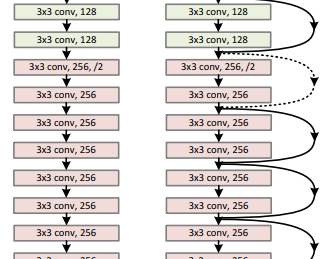
\includegraphics[width=5cm]{charts/resnet.png} }}%
    \qquad
    \subfloat[A building Residual block]{{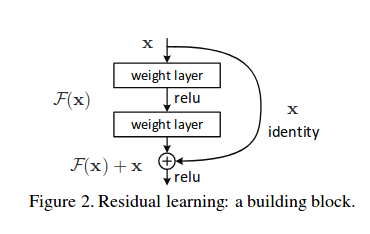
\includegraphics[width=5cm]{charts/resnet1.png} }}%
    \caption{There are different versions of ResNet indicating the number of layers ranging from 20 to 1202. An ensemble of 6 models with different depths achieves a top-5 validation error of 3.57\% and wins the 1st place in ILSVRC-2015. }%
    \label{fig:resnet}%
\end{figure}

\section{Semantic Word Embedding}
Understanding the semantic meaning of words has been playing the key role in modern Natural Languague Processing problems. Before the emergence of Word Embedding models, we used bag-of-word to represent features (e.g. TF-IDF \cite{tfidf}) of words, which tend to be high dimensional while not preserving the semantic relationships between entities. The term \textit{word embedding} was originally coined by Bengio et al. \cite{bengio2003} in 2003 who trained them in a neural language model and named the process as \emph{learning a distributed representation for words}. Their model takes a sequence of words and try to predict the next word thus implicitly encoding the semantic relationships in a layer called \emph{embedding}. 

\begin{figure}
\centering
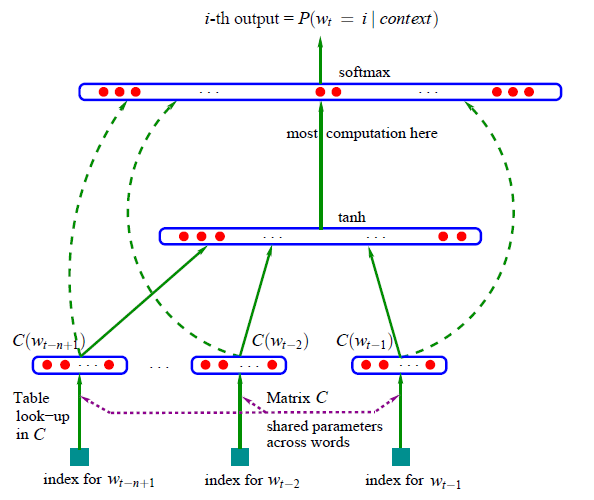
\includegraphics[scale=0.5]{charts/bengio_language_model.png}
\caption{Classic neural language model described in \cite{bengio2003}.}
\end{figure}

Ten years after the initial idea of learning word representations using neural network, Mikolov et al. \cite{word2vec} recommended two architectures for this problem, which is called Word2Vec. Not only these architectures are computationally less expensive than previous models, but the proposed training strategy, especially Negative Sampling, are way more effective, making Word2Vec the most popular embedding models being used today. 
\begin{figure}
\centering
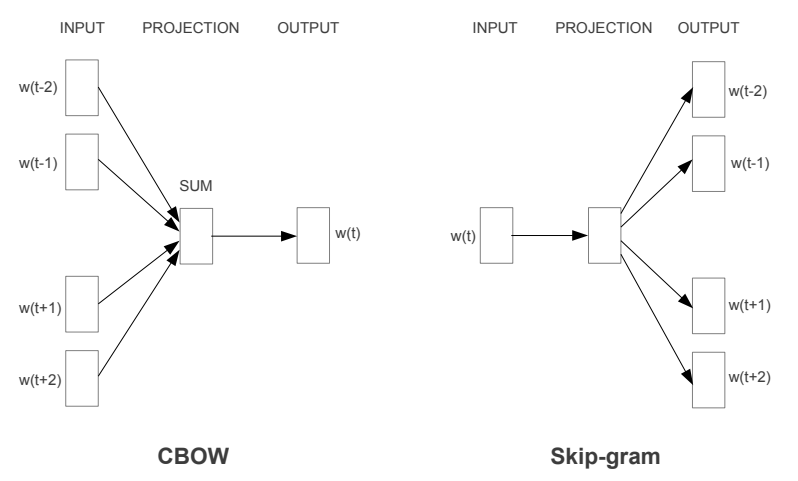
\includegraphics[scale=0.5]{charts/word2vec.png}
\caption{Two architectures for learning word embedding proposed in Word2Vec. In CBOW, rather than feeding $n$ previous words into the model, the model receives a window of $n$ words around the target word $w_t$ at each time step $t$. Meanwhile, Skip-gram does the opposite thing when using the centre word to predict the surrounding words.}
\end{figure}

Following the success of Word2Vec, FastText \cite{fasttext} was proposed by FAIR to further learn the representations of words which are rare or even out of learning corpus. Instead of directly learning a vector representation for a word (as with word2vec), FasText learns a representation for each \textit{character n-gram}. In other words, each word is represented as a bag of character n-grams, so the overall word embedding is a sum of these character n-grams. For that reason, FastText is more of a general framework of representing word embeddings and can be applied to different text problems.

\begin{figure}
\centering
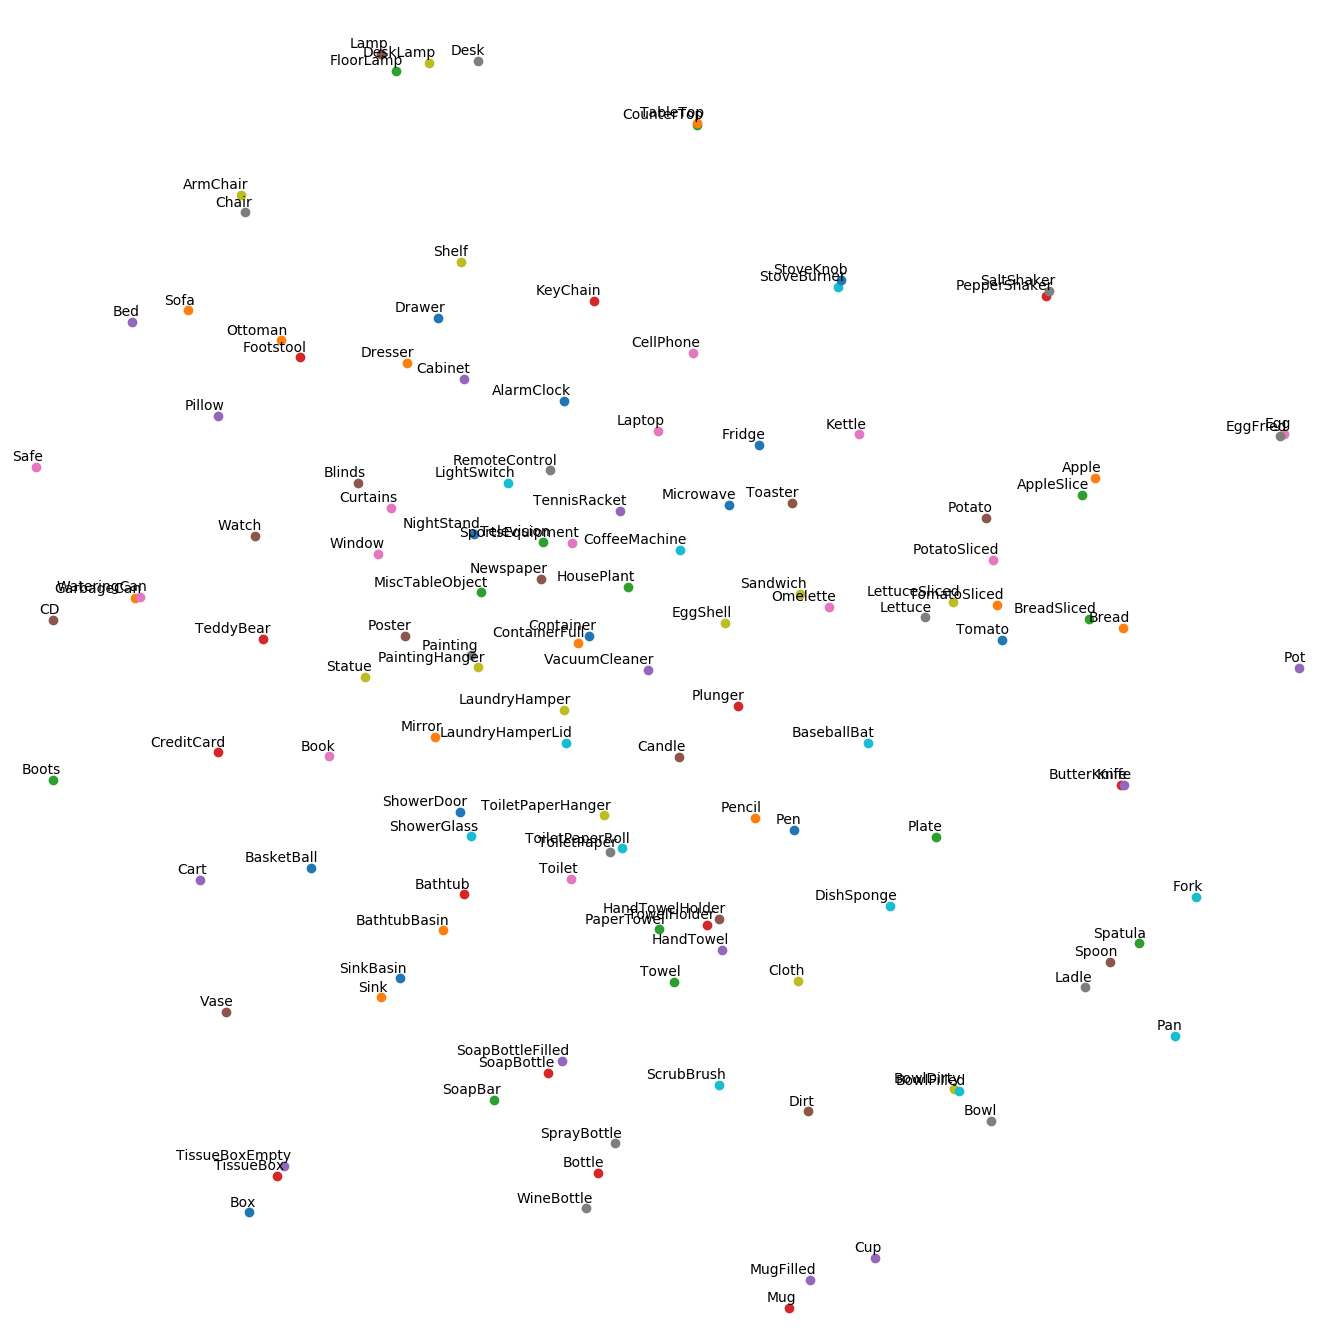
\includegraphics[scale=0.3]{charts/tsne.png}
\caption{FastText embeddings of target names. The vector dimension is reduced from 300 to 200 using T-sne \cite{tsne} algorithm.}
\end{figure}

\section{Graph Convolutional Network}

GCN is a very powerful neural network architecture for doing machine learning on graphs. More formally, given a graph $\mathcal{G}=(\mathcal{V}, \mathcal{E})$, a GCN takes as input:
\begin{itemize}
\item A $N\times D$ feature matrix $X$, holding features of every node $x_i$, where $N$ is the number of nodes, $D$ is the number of features of each node.
\item An adjacency matrix $A$ representing the graph structure.
\end{itemize}
and produces a node-level output $Z$ which is an $N\times F$ feature matrix, where $F$ is the number of features per output node. 

\begin{figure}
\centering
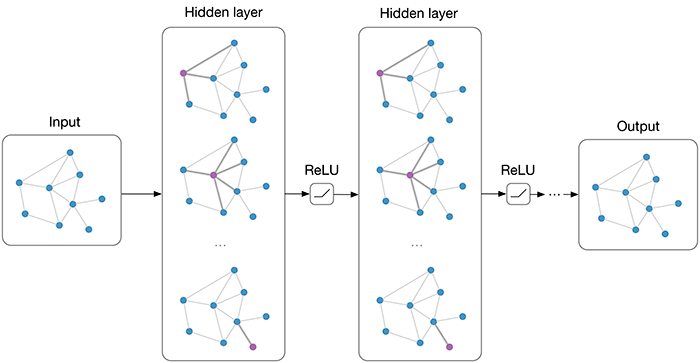
\includegraphics[scale=0.5]{charts/gcn_web.png}
\caption{Multi-layer Graph Convolutional Network (GCN) with first-order filters.}
\end{figure}

Every neural network layer of GCN functions as the following formula:
\begin{align}
H^{(l+1)} &= f(H^{(l)}, A)\,, \label{gcn_eq}
\end{align}
where $H^{(0)} = X$ and $H^{(L)} = Z$, $L$ is the number of layers. One simple yet common choice for function $f$ in \ref{gcn_eq} is 

\begin{align}
f(H^{(l)}, A) &= \sigma\left( AH^{(l)}W^{(l)}\right) \, ,
\end{align}

where $W^{(l)}$ is a weight matrix for the $l$-th layer and $\sigma(\cdot)$ is a non-linear activation function like the ReLU \cite{relu}. Despite the simplicity, this architecture is so powerful that even a randomly initiated 2-layer GCN can produce useful feature representations of nodes, including semantic relationships. In fact, to further enhance the power of GCN and eliminate some existing limitations,  Kipf \& Welling \cite{gcn} suggested the following propagation rule:

\begin{align}
f(H^{(l)}, A) &= \sigma\left( \hat{D}^{-\frac{1}{2}}\hat{A}\hat{D}^{-\frac{1}{2}}H^{(l)}W^{(l)}\right) \, ,
\end{align}

where $\hat{A} = A + I$, $I$ is the identity matrix and $\hat{D}$ is the diagonal node degree matrix of $\hat{A}$.




\newpage\cleardoublepage
\chapter{Proposed method}

Some mathematics formula $$F(x) = \argmax_{y \in GEN(x)} w \cdot f(x, y)$$\newpage\cleardoublepage
\chapter{Evaluation}
In this chapter, ...\newpage\cleardoublepage
\chapter{Conclusion}
In this chapter, ...\newpage\cleardoublepage

%Adding the acronyms to the glossary without displaying them here:
\glsadd{cnn}

\printglossaries

\nocite{*}
\bibliography{references}\newpage\cleardoublepage
\bibliographystyle{plain}
\end{document}